\section*{Backup slides}

\begin{frame}
	\frametitle{Bands flattening: a signature of Mott localisation}
	\begin{columns}
		\column{0.4\linewidth}
		\begin{figure}
			\centering
			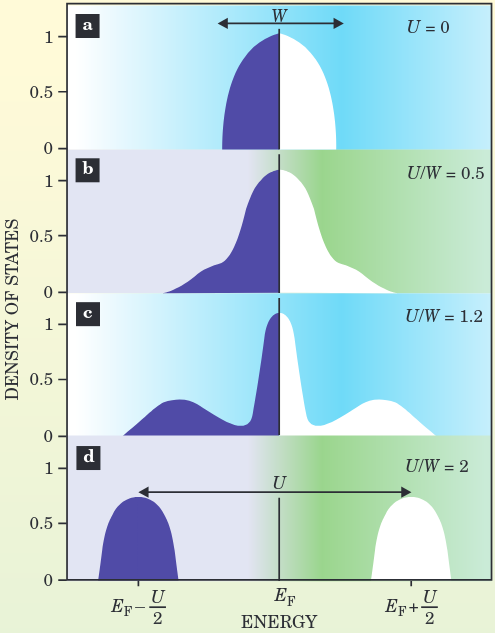
\includegraphics[width=\columnwidth]{sections/introduction/dos.png}
			\caption*{Gabriel Kotliar and Dieter Vollhardt, 2004. \textbf{Physics Today 57 (March): 53–59}.}
		\end{figure}
		\column{0.5\linewidth}
		As we increase the ratio $U/t$, the many-body DoS undergoes a transition:
		\begin{enumerate}
			\item[(a)] Free model, conventional DoS;
			\item[(b)] Weak coupling, large coherent peak;
			\item[(c)] Intermediate coupling, \textbf{narrow coherent peak};
			\item[(d)] Strong coupling, lower and upper Hubbard bands.
		\end{enumerate}
		\DownImplication
		Localisation = flattening of bare bands.
	\end{columns}
\end{frame}

\begin{frame}
	\frametitle{The iterative algorithm (iHF)}
	\begin{columns}
		\column{0.45\linewidth}
		The HF solution is the \textbf{fixed point} of a non-linear map $\mathrm{A}$,
		\[
		\mathrm{A}(\mathbf{v}) = \mathbf{v} \, .
		\]
		\DownImplication
		\textbf{Strategy}: ``follow'' the map up to the fixed point,
		\[
		\mathbf{v}_{i+1} \equiv g \mathrm{A}(\mathbf{v}_i) + (1-g) \mathbf{v}_i \, .
		\]
		with $i>0$, $g \in [0,1]$.
		\DownImplication
		\column{0.45\linewidth}
		\begin{figure}
			\centering
			
\includegraphics[width=\columnwidth]{/home/nepero27178/Thesis/EHM-HF/Project/src/labs/attractor/example-attractor-ink.pdf}
			\caption*{Example path for the AF phase.}
		\end{figure}
	\end{columns}
	\textbf{Convergence criterion}:
	\[
	\forall j \quad\colon\quad
	\left[ \mathbf{v}_{i+1} - \mathbf{v}_i \right]_j < \Delta v_j \, ,
	\]
	with $\Delta \mathbf{v}$ the vector of tolerances.
\end{frame}